\documentclass{article}
\usepackage[margin=1in]{geometry}
\usepackage{setspace}
\usepackage{graphicx}
\usepackage{amsmath}
\usepackage{amssymb}
\usepackage{booktabs}
\usepackage{multirow}
\usepackage{tikz}
\usetikzlibrary{arrows.meta}
\usepackage[colorlinks=true,linkcolor=blue,citecolor=blue,urlcolor=blue]{hyperref}  % load last

\numberwithin{equation}{section}   % equations numbered (2.13), where "2" is the section number

\def\DDS{{\rm DDS}}
\def\DD{{\rm DD}}
\def\TDS{{\rm TDS}}
\def\LDS{{\rm LDS}}
\def\LS{{\rm LS}}
\def\LAG{{\rm LAG}}
\def\nn{\nonumber}

% These notes are split across three PDFs, compiled independently from
% notes/dedispersion.tex, notes/detrending.tex, notes/variance_map.tex.
% Everything above this comment is deliberately IDENTICAL in all three sources,
% so that a section can be moved between them without touching the preamble.
%
% A \ref cannot cross documents, so a pointer into a companion PDF names its
% section in prose instead: \ddnotes{Subband search} renders as
% [dedispersion.pdf, "Subband search"]. Each source defines the macros for the
% other two documents (either may be unused at any given moment). The argument
% must reproduce a section or subsection title of the companion verbatim.
\newcommand{\dtnotes}[1]{{\em detrending.pdf}, ``#1''}
\newcommand{\vmnotes}[1]{{\em variance\_map.pdf}, ``#1''}

\title{Notes on the ``pirate'' dedisperser: tree dedispersion}
\author{Kendrick Smith}

\begin{document}

\maketitle

\tableofcontents

\setstretch{1.05}   % spacing between lines
\setlength{\parskip}{2.5pt}  % spacing between paragraphs

\clearpage

\section{Tree dedispersion}
\label{sec:tree_dedispersion_top}

\subsection{Tree gridding kernel}
\label{sec:gridding}

Our starting point for tree dedispersion is a shape $(N_{\rm freq}, N_{\rm time})$ array representing channelized intensity time series. We do not assume that frequency channels are evenly spaced (in CHORD we use unequal spacing).
We want to search this array for FRBs with delay $\propto \nu^{-2}$.

The first step is a ``tree gridding'' kernel which changes variables so that the delay is linear (i.e.~the FRB dispersion sweep looks like a straight line).
The input of the tree gridding kernel is a shape $(N_{\rm freq}, N_{\rm time})$ array, and the output is a shape $(N_{\rm tree}, N_{\rm time})$ array, where $N_{\rm tree}=2^r$.
The parameter $r$ is the tree dedispersion ``rank'' and is specified in a config file.

The leading axis of the input array represents frequency channels, and will be indexed by $0 \le F < N_{\rm freq}$.
The leading axis of the output array represents a reparameterized frequency channel (``tree-freq'' channel for short), and will be indexed by $0\le f < 2^r$.
Conceptually, the tree gridding kernel just reparameterizes the frequency axis (i.e.\ the time axis is a spectator.)

The tree gridding kernel also takes an auxiliary array \verb|channel_map|, which describes the mapping between frequency channels $0 \le F < N_{\rm freq}$ and tree-freq channels $0 \le f < N_{\rm tree}$.
The array \verb|channel_map| has length $N_{\rm tree}+1$, and its entries are (in general non-integer) frequency-channel indices in the range $[0, N_{\rm freq}]$.
Writing $c_f$ for the $f$-th entry, tree-freq channel $f$ is defined to occupy the half-open interval of frequency channels
\begin{equation}
I_f = \big[\, c_{f+1},\ c_f \,\big), \qquad 0 \le f < N_{\rm tree},
\end{equation}
i.e.~consecutive entries give the lower and upper edges of each tree-freq channel.
The entries are fixed by the dispersion geometry: the tree-freq channels are equally spaced in the dispersion variable $x \equiv \nu^{-2}$ (this is the change of variables that linearizes the delay), so the $f$-th edge sits at
\begin{equation}
x_f = \nu_{\rm hi}^{-2} + \frac{f}{N_{\rm tree}}\left(\nu_{\rm lo}^{-2} - \nu_{\rm hi}^{-2}\right),
\end{equation}
and $c_f$ is the frequency-channel index of the frequency $\nu_f = x_f^{-1/2}$, where the index increases with frequency, running from $0$ at the band bottom $\nu_{\rm lo}$ to $N_{\rm freq}$ at the band top $\nu_{\rm hi}$.
In particular $c_0 = N_{\rm freq}$ and $c_{N_{\rm tree}} = 0$, so \verb|channel_map| is monotonically {\em decreasing} ($c_{f+1} < c_f$).
We store it in double precision, since the gridding weights below are obtained by differencing adjacent entries, which loses relative precision.

The details of the tree gridding kernel are as follows.
Each output tree-freq channel $f$ is a weighted sum of the input frequency channels whose bins overlap the interval $I_f = [c_{f+1}, c_f)$:
\begin{equation}
{\rm out}[f] = \sum_{F=0}^{N_{\rm freq}-1} w_{fF}\, {\rm in}[F],
\end{equation}
where ${\rm in}[F]$ and ${\rm out}[f]$ are length-$N_{\rm time}$ time series, and the same weights are applied at every time sample (the time axis is untouched).
The weight $w_{fF}$ is the length of the overlap between the tree-freq channel interval $I_f$ and the unit-width frequency bin $[F, F+1)$:
\begin{equation}
w_{fF} = \max\!\big(\,0,\ \min(c_f,\, F+1) - \max(c_{f+1},\, F)\,\big).
\end{equation}
A frequency channel lying entirely within $I_f$ contributes with weight $1$, while a channel straddling an edge of $I_f$ contributes a fractional weight.
Because the intervals $I_f$ tile $[0, N_{\rm freq}]$, the weights of any fixed input channel sum to one, $\sum_f w_{fF} = 1$; the gridding kernel is thus a delay-linearizing rebinning of the frequency axis that conserves total intensity, $\sum_f {\rm out}[f] = \sum_F {\rm in}[F]$.

Note that the tree gridding kernel is a monotone {\em decreasing} reindexing operation.
Thus, to search for FRBs with positive dispersion (lowest frequencies arise last), we want to search over lines in the tree array with positive slope (highest tree-freq channels arrive last).

\subsection{Tree dedispersion}
\label{sec:tree_dedispersion}

After the tree gridding kernel, the next step is ``tree dedispersion'', which searches for straight lines with $0\le \mbox{slope} \le 1$.
(The extension to slope $>1$ will be discussed in a future section, along with more details such as subband searches, early triggers, and peak-finding.)

The dedispersion input array has shape $(2^r, N_{\rm time})$, where the leading axis is ``tree-freq'' (see above).
Straight lines will be parameterized by an integer $0 \le d < 2^r$, representing
the delay (in time samples) between the lowest and highest tree-freq channel,
and a time index $t$ representing the arrival time in the {\em highest} tree-freq channel
(i.e. the {\em latest} arrival time).
Thus, the dedispersion output array also has shape $(2^r, N_{\rm time})$, where the first axis represents a delay (or DM).\footnote{Frequently in the code (but not in these notes), it's convenient to use a {\em bit-reversed} delay index $0 \le d_{\rm rev} < 2^r$. (This turns out to allow some array operations to operate ``in place'', facilitating parallelization.)}

Tree dedispersion is a composition of functions:
\begin{equation}
\big( \mbox{Input array} \big)
  \overset{\DDS(0)}{\longrightarrow} \big( \mbox{Intermediate array} \big)
  \overset{\DDS(1)}{\longrightarrow} \cdots 
  \overset{\DDS(r-1)}{\longrightarrow}
\big( \mbox{Output array} \big)
\label{eq:DD_composition}
\end{equation}
where the function $\DDS(k)$ (``dedispersion step $k$'') is described as follows:

\begin{itemize}

\item
The $\DDS(k)$ input array is a shape $(2^{r-k}, 2^k, N_{\rm time})$ array.
The first axis represents a coarse frequency channel.
Each coarse-freq channel $f$ corresponds to a block of $2^k$ tree-freq channels
in the original tree input array:
\begin{equation}
2^k \, f \le (\mbox{tree-freq index}) < 2^k (f+1)  \label{eq:coarse_freq}
\end{equation}
The second axis represents a delay $0 \le d < 2^k$ within the coarse-freq channel
(\ref{eq:coarse_freq}). As $k$ increases, the coarse-freq channels double in width,
and we need twice as many delay indices to cover the range $0 \le (\mbox{slope}) \le 1$.

The time index represents an arrival time at the largest tree-freq channel
in the coarse-freq channel (\ref{eq:coarse_freq}), i.e.~the latest arrival time within the coarse-freq channel.

\item The $\DDS(k)$ operation is defined by:

\begin{align}
{\tt out}[f,2d,t] &= \frac{1}{\sqrt{2}} 
  \big( {\tt in}[2f,d,t-d] + {\tt in}[2f+1,d,t] \big) \nn \\
{\tt out}[f,2d+1,t] &= \frac{1}{\sqrt{2}} 
  \big( {\tt in}[2f,d,t-d-1] + {\tt in}[2f+1,d,t] \big)
\end{align}

\item
As formulated above, tree dedispersion can lead to negative time indices.
By default, \verb|in[...,t]| with $t<0$ is defined to be zero.
(In the real-time system, we run tree dedispersion in an ``incremental'' context where a negative time index should be interpreted as a reference to data received in a previous time chunk.)

\item The $\DDS(0)$ input array is sometimes reshaped from $(2^r,1,N_{\rm time})$
 to $(2^r,N_{\rm time})$, and the $\DDS(r-1)$ output array is sometimes reshaped
 from $(1,2^r,N_{\rm time})$ to $(2^r,N_{\rm time})$.
 Thus, we think of the entire tree dedispersion operation (\ref{eq:DD_composition}) as having input and output shapes $(2^r, N_{\rm time})$.

\end{itemize}

\par\noindent
We define $\DD(r)$ (``rank-$r$ dedispersion'') to be the composition of all $r$ steps in Eq.\ (\ref{eq:DD_composition}):
\begin{equation}
\DD(r) = \DDS(r-1) \circ \cdots \circ \DDS(0)  \label{eq:DD_DS}
\end{equation}

\subsection{Subband search}
\label{sec:subband_search}

So far, we have described a search for FRBs which cover the full tree-freq range $0 \le f < 2^r$.
This would be suboptimal since real FRBs do not always cover the full frequency range.
Next, we introduce a ``sub-band'' search for searching a configurable set of subbands.

\subsubsection{Parameterization of subbands}

Our dedispersion config files contain a length-$(R+1)$ integer-valued array of subband counts $C_l$.\footnote{In 
the code, $R$ is denoted {\tt pf\_rank}, $l$ is denoted {\tt pf\_level}, and $C_l$ is denoted {\tt frequency\_subband\_counts}.}
Here $0 \le R \le r$, where $r$ is the tree rank.
The counts $C_l$ parameterize a set of subbands as follows:
\begin{itemize}
\item Frequency subbands are indexed by a pair $(l,s)$ where $0 \le l \le R$ and $0 \le s < C_l$.
We will sometimes ``flatten'' the pair $(l,s)$ into a single subband index $0 \le n < N$, where
\begin{equation}
N \equiv \sum_{l=0}^R C_l
\end{equation}
is the total number of subbands. 
(In the code, $n$ and $N$ are denoted by the same symbols, e.g.\ $N$ is {\tt FrequencySubbands::N}.)
\item Level $l=0$ is special: subband $(0,s)$ corresponds to tree-freq range
\begin{equation}
2^{r-R} s \le \mbox{(tree-freq index)} < 2^{r-R} (s+1)  \label{eq:subband_l0}
\end{equation}
\item At levels $l>0$, subband $(l,s)$ corresponds to tree-freq range
\begin{equation}
2^{r-R+l-1} s \le \mbox{(tree-freq index)} < 2^{r-R+l-1} (s+2)  \label{eq:subband_l1}
\end{equation}
Thus, level 0 consists of non-overlapping bands whose fractional width is $1/2^R$.
Levels $l>0$ consist of bands whose fractional width is $1/2^{R-l}$, and overlap by a factor 2.
\item
To avoid ``overflowing'' the band, $C_l$ must satisfy
\begin{equation}
0 \le C_l \le \begin{cases}
2^R & \mbox{for } l=0 \\
2^{R-l+1}-1 & \mbox{for } l>0
\end{cases}
\end{equation}
A level with $C_l=0$ is allowed, and simply contributes no subbands.
We require $C_R=1$, i.e.~we always search the full frequency band.
The case $C_l=\{1\}$ (with $R=0$) corresponds to disabling subbands, and only searching the full band.
\item The details of this scheme, including the ``specialness'' of level $l=0$, are
dictated by convenience in the GPU kernel.
\item To {\em interpret} the $C_l$ already in a config file, run \verb|pirate_frb show dedisperser -cv|.
For example, for $C_l=[5,9,7,3,1]$ this prints:
\begin{verbatim}
# In this config, there are 25 top-level frequency subband(s):
#   pf_level=0: [948.7,1500.0], [750.0,948.7], [639.6,750.0], [566.9,639.6], [514.5,566.9]
#   pf_level=1: [750.0,1500.0], [639.6,948.7], [566.9,750.0], [514.5,639.6], [474.3,566.9],
#               [442.3,514.5], [416.0,474.3], [393.9,442.3], [375.0,416.0]
#   pf_level=2: [566.9,1500.0], [474.3,750.0], [416.0,566.9], [375.0,474.3], [344.1,416.0],
#               [319.8,375.0], [300.0,344.1]
#   pf_level=3: [416.0,1500.0], [344.1,566.9], [300.0,416.0]
#   pf_level=4: [300.0,1500.0]
\end{verbatim}
\item To {\em create} a $C_l$ array with a given max $\Delta(\log \nu)$, run \verb|pirate_frb dev make_subbands|.
For example, \verb|pirate_frb dev make_subbands 300 1500 0.1 -r 4| gives $C_l=[5,9,7,3,1]$.
These subbands are shown visually in Figure \ref{fig:subbands}.
\end{itemize}
\begin{figure}
\centering
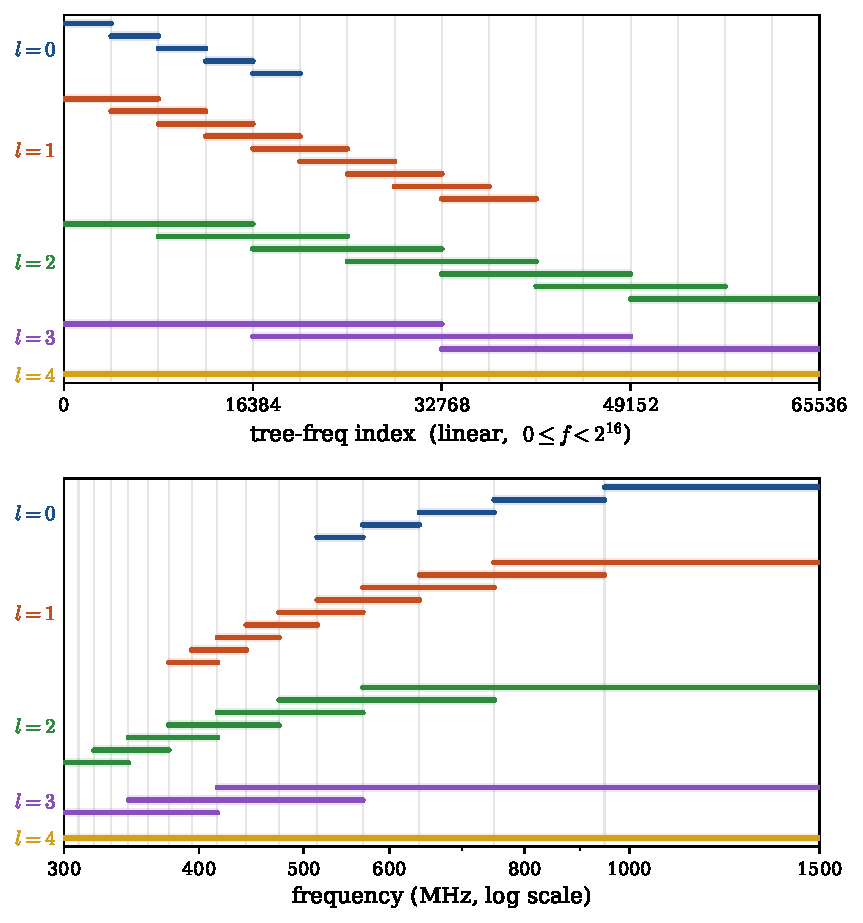
\includegraphics[width=\textwidth]{figs/chord_subbands.pdf}
\caption{Frequency subbands in a CHORD config with {\tt frequency\_subband\_counts=[5,9,7,3,1]}).
The top panel shows the subbands in tree-freqs (where they are ``naturally'' defined) and the bottom
panel shows the conversion to physical frequency $\nu$ in MHz. Note that the conversion between tree-freqs
and $\nu$ is monotone decreasing.}
\label{fig:subbands}
\end{figure}

\subsubsection{Subbanded dedispersion}
\label{sssec:subbanded_dedispersion}

Subbanded dedispersion is an operation whose input array is the same as ordinary (non-subbanded) tree 
dedispersion (\ref{sec:tree_dedispersion}), i.e.\ a shape $(2^r, N_{\rm time})$ array where the first index is tree-freq.
The output array has shape $(2^{r-R}, M, N_{\rm time})$, where $M$ is the number of ``multiplets'':
\begin{equation}
M \equiv \sum_{l=0}^R 2^l C_l  \label{eq:multiplet_def}
\end{equation}
The code requires $R \le 4$ ({\tt constants::max\_peak\_finding\_rank}), so saturating the bounds
on $C_l$ above gives $C_l = [16,15,7,3,1]$, and hence $N \le 42$ and $M \le 114$.

Each subband $(l,s)$ ``owns'' a shape $(2^{r-R}, 2^l, N_{\rm time})$ subarray of the output.
The first two axes correspond to $2^{r-R+l}$ dispersion delays across the subband, split into a ``coarse'' index
$0 \le d_{\rm hi} < 2^{r-R}$ and a ``fine'' index  $0 \le d_{\rm lo} < 2^l$.
(This index-splitting ensures that the combined output of all subbands is a regular $(2^{r-R}, M, N_{\rm time})$ array,
rather than a ``ragged'' object.)

Conceptually, subband dedispersion works as follows.
For each subband $(l,s)$, we apply tree dedispersion to the appropriate tree-freq range (either Eq.\ (\ref{eq:subband_l0}) 
or (\ref{eq:subband_l1})). We also apply a time lag so that the time index corresponds to the extrapolated arrival time at 
the highest tree-freq in the full band, not the highest tree-freq in the subband.
For an efficient implementation, we run tree dedispersion as usual (Eq.\ \ref{eq:DD_composition}), and extract per-subband
dedispersion outputs from intermediate arrays ``on the fly'', rather than dedispersing each subband ``from scratch''.

Formally, the details are as follows:

\begin{itemize}

\item {\bf Case 1: $l=0$ or even $s$.}
In this case, the subband corresponds to an ``aligned'' tree-freq range of the form:
\begin{equation}
2^{r-R+l} f \le \mbox{(tree-freq index)} < 2^{r-R+l}(f+1) \hspace{1cm} \mbox{(where $0 \le f < 2^{R-l}$)}
\end{equation}
where the coarse-freq index $f$ is given by:
\begin{equation}
f = \begin{cases} s & \mbox{if } l=0 \\ s/2 & \mbox{if } l > 0 \end{cases}
\end{equation}
The subband owns a shape $(2^{r-R}, 2^l, N_{\rm time})$ subarray of the output (denote by \verb|out|).

In this case, the per-subband dedispersion outputs already arise as intermediates in tree dedispersion
(Eq.\ \ref{eq:DD_composition}); we just need to apply a time lag.
Let \verb|tmp| be the output array of $\DDS(k-1)$, where $k=r-R+l$. 
Then \verb|tmp| has shape $(2^{R-l}, 2^{r-R+l}, N_{\rm time})$.
To populate the \verb|out| array, we slice/reshape \verb|tmp| and apply time lags:
\begin{equation}
{\tt out}\big[ d_{\rm hi}, d_{\rm lo}, t \big] = {\tt tmp}\big[ f, d, t - T \big]
\end{equation}
where on the RHS we define:
\begin{equation}
d \equiv d_{\rm hi} 2^l + d_{\rm lo}   \hspace{1.5cm} T \equiv d_{\rm hi} 2^l (2^{R-l}-1-f)
\label{eq:case1_lags}
\end{equation}

\item {\bf Case 2: $l>0$ and odd $s$.}
In this case, the subband corresponds to a ``half-aligned'' tree-freq range of the form:
\begin{equation}
2^{r-R+l-1} (2f+1) \le \mbox{(tree-freq index)} < 2^{r-R+l-1}(2f+3) \hspace{1cm} \mbox{(where $0 \le f < 2^{R-l}-1$)}
\end{equation}
where the coarse-freq index $f$ is given by $f \equiv (s-1)/2$.
The subband owns a shape $(2^{r-R}, 2^l, N_{\rm time})$ subarray of the output (denote by \verb|out|).

This case is a little more complicated, since the per-subband dedispersion outputs are ``one dedispersion step away''
from the intermediate arrays in tree dedispersion.
Let \verb|tmp| be the output array of $\DDS(k-1)$, where $k=r-R+l-1$. 
Then \verb|tmp| has shape $(2^{R-l+1}, 2^{r-R+l-1}, N_{\rm time})$.
\begin{align}
{\tt out}\big[ d_{\rm hi}, 2 d_{\rm lo}, t \big] 
  &= \frac{1}{\sqrt{2}} \Big( {\tt tmp}\big[ 2f+1, d, t - T_0 - d \big] + {\tt tmp}\big[ 2f+2, d, t - T_0 \big] \Big) \nn \\
{\tt out}\big[ d_{\rm hi}, 2 d_{\rm lo} + 1, t \big] 
  &= \frac{1}{\sqrt{2}} \Big( {\tt tmp}\big[ 2f+1, d, t - T_1 - d - 1 \big] + {\tt tmp}\big[ 2f+2, d, t - T_1 \big] \Big) 
\end{align}
where on the RHS we define:\footnote{In 
 Eqs.\ (\ref{eq:case1_lags}), (\ref{eq:case2_lags}),
 we defined delays $T,T_0,T_1$ as follows:
 \begin{equation}
 T = d_{\rm hi} 2^l (2^{R-l}-1-f) \hspace{1.5cm}
   T_0 = T_1 = d_{\rm hi} 2^{l-1} (2^{R-l+1} - 2f - 3)
 \end{equation}
 These definitions reflect what is currently implemented (in the GPU kernels and in {\tt ReferenceTree}), 
 but in hindsight these definitions may make more sense:
 \begin{equation}
  T = (d_{\rm hi} 2^l + d_{\rm lo}) \,(2^{R-l}-1-f)
 \hspace{1cm}
 T_0 = (d_{\rm hi} 2^{l-1} + d_{\rm lo}) \, (2^{R-l+1}-2f-3)
 \hspace{1cm}
 T_1 = T_0 + (2^{R-l}-f-2)
\end{equation}
We may switch the code to this convention in the future.}
\begin{equation}
d \equiv d_{\rm hi} 2^{l-1} + d_{\rm lo}
  \hspace{1.5cm} T_0 = T_1 = d_{\rm hi} 2^{l-1} (2^{R-l+1} - 2f - 3)
\label{eq:case2_lags}
\end{equation}
(Warning: the quantities $f,k,d_{\rm lo}$ have slightly different meanings in cases 1 and 2!)

\end{itemize}
Note that subband dedispersion includes the full band (via $C_R=1$), but the full-band output array is
``reshaped'' to $(2^{r-R}, 2^R, N_{\rm time})$, whereas in the previous section it had shape $(2^r, N_{\rm time})$.

\subsection{Peak-finding}
\label{sec:peak_finding}

The final stage of the dedispersion transform is {\em peak-finding}.
For now, we give a partial description -- a future version of the notes will describe
peak-finding in more detail.
The input is the shape-$(2^{r-R}, M, N_{\rm time})$ array from the previous section.
The output is a shape-$(2^{r-R-K}, N_{\rm time}/T_{\rm ds})$ array, where $T_{\rm ds}$ 
is a time downsampling factor, and $K\ge 0$ allows additional DM downsampling.
Conceptually, peak-finding is 3 steps:
\begin{itemize}
\item For each $(d_{\rm hi}, m)$, the input array is a 1-d time series.
We convolve the time series with $P$ peak-finding kernels, described below, to
obtain a shape $(2^{r-R}, M, N_{\rm time}, P)$ array.
\item We apply weights that depend on $(d_{\rm hi}, m, p)$, to normalize the array 
so that each array element has variance 1. (Thus, array elements are normalized to
``sigmas''.)
\item We downsample the array to shape $(2^{r-R-K}, N_{\rm time}/T_{\rm ds})$.
Downsampling is done with ``max'' rather than addition, so each array element
corresponds to max detection significance over all downsampled parameters.
\end{itemize}
In implementation, these 3 steps are coalesced into one GPU kernel for speed (and also
coalesced with the final stages of tree dedispersion), e.g.\ the shape $(2^{r-R}, M, N_{\rm time}, P)$
array is never ``materialized'' in GPU memory.\footnote{Another comment on implementation. A
{\tt PeakFindingKernel} takes $K$ as the constructor argument {\tt PeakFindingKernelParams::xdm\_rank};
it reads a $(2^{r-R}, M)$ array and reduces over the low $K$ bits of the first index itself.
A {\tt CoalescedDdKernel2} instead ``chooses'' $K = \mbox{\tt rank1} - R$ from its own ranks,
and asserts that the caller's {\tt xdm\_rank} agrees. See comments in code.}

\subsubsection{Peak-finding kernels}

There is always one profile ($p=0$) consisting of a single unsmoothed sample. The remaining
kernels are organized into $\Lambda \equiv \log_2 W_{\rm max}$ {\em levels} $0 \le \lambda < \Lambda$,\footnote{We use $\lambda$ and $\Lambda$ here to avoid ambiguity with the subband level $l$ in \S\ref{sec:subband_search}. In the code, the level index appears as {\tt l} in {\tt PfVarianceConvolver.peak\_finding\_kernels()} and as {\tt lgw} in the kernel generator {\tt PeakFinder}.} where
$W_{\rm max}$ (a power of two) is the config parameter \verb|max_kernel_width|, and each level
contributes three profiles. The total number of profiles is therefore
\begin{equation}
P = 3 \log_2 W_{\rm max} + 1.
\end{equation}
The edge case $W_{\rm max}=1$ is allowed: there are then no levels, and the single sample
$p=0$ is the only profile.
The building block at level $\lambda$ is the {\em unnormalized running boxcar sum} of width $2^\lambda$,
\begin{equation}
b_\lambda[t] \equiv \sum_{i=0}^{2^\lambda - 1} x[t-i],
\end{equation}
computed by the recursion
\begin{equation}
b_0[t] = x[t], \qquad b_{\lambda+1}[t] = b_\lambda[t] + b_\lambda[t - 2^\lambda].
\label{eq:boxcar_recursion}
\end{equation}
Note that (\ref{eq:boxcar_recursion}) is a {\em plain sum}: there is no $1/\sqrt2$ in the boxcar
downsampling. (All normalization is deferred to the weights.)

At each level $\lambda$ we form up to four kernels, denoted $h_{\lambda,q}$ where $0\le q \le 3$:
\begin{align}
h_{\lambda,0} &= [\,\underbrace{1,\dots,1}_{2^\lambda}\,] \nn \\
h_{\lambda,1} &= [\,\underbrace{1,\dots,\dots,1}_{2^{\lambda+1}}\,] \nn \\
h_{\lambda,2} &= [\,\underbrace{\tfrac12,\dots}_{2^\lambda},\ \underbrace{1,\dots}_{2^\lambda},\ \underbrace{\tfrac12,\dots}_{2^\lambda}\,] \nn \\
h_{\lambda,3} &= [\,\underbrace{\tfrac12,\dots}_{2^\lambda},\ \underbrace{1,\dots,\dots,1}_{2^{\lambda+1}},\ \underbrace{\tfrac12,\dots}_{2^\lambda}\,]
\end{align}
The profile index $0\le p < P$ is related to $(\lambda,q)$ by $p = 3\lambda + q$, with the special value $p = 0$ for
$(\lambda,q) = (0,0)$. Thus level $\lambda$ contributes $p = 3\lambda+1, 3\lambda+2, 3\lambda+3$, and $p=0$ (i.e.\
$h_{0,0} = [1]$, the single sample above) sits outside the levels. The single-boxcar kernel $h_{\lambda,0}$ never
appears for $\lambda > 0$, since $h_{\lambda,0} = b_\lambda = h_{\lambda-1,1}$ would be redundant. So one may equally
say that level $0$ contributes $p=0,1,2,3$ and each higher level contributes three profiles; the two descriptions
agree except at $W_{\rm max}=1$, where there are no levels at all and $p=0$ is the only profile.

\subsection{Time-downsampled trees and early triggers}
\label{sec:downsampled_early}

So far, we have described a single {\tt DedispersionTree} which searches up to slope 1 (i.e.~full-band dispersion delay equal to $2^r$ time samples), and ``triggers'' when the pulse arrives at the lowest frequency (highest tree-freq).
It will be useful to define a larger {\tt Dedisperser} object, consisting of multiple trees, as follows:

\begin{itemize}

\item {\bf Downsampled trees} in order to search to higher DM. 
If we time-downsample the data by a factor $2^\gamma$, and run rank-$r$ dedispersion as usual, then we can search to a max dispersion delay which is larger by a factor $2^\gamma$.
When we time-downsample by a factor $2^\gamma$, we add time samples and multiply by $2^{-\gamma/2}$, in order to leave the variance unchanged (assuming uncorrelated samples).

If $\gamma > 0$, then we only keep the upper half (in delay) of the dedispersion output, since the lower half was already searched by primary tree $(\gamma-1)$.
Thus, each value of $\gamma$ corresponds to a different DM range, ordered from low to high DM.

\item {\bf Early triggers} in order to reduce triggering latency, especially at high DM. 
By default, we only trigger when the pulse arrives at the highest tree-freq $f=2^r$ (i.e.\ lowest radio frequency).
If we run parallel tree dedispersion over the lowest $2^{r-e}$ tree-freqs (i.e.\ highest radio frequencies),
then the triggering time will be smaller by a factor $2^e$.
This comes at the expense of losing low frequencies, so not all bursts will be detected in the early trigger.

\end{itemize}

\par\noindent
The {\tt Dedisperser} consists of multiple trees parameterized by $(\gamma,e)$.
In the dedispersion config file, the syntax is (from {\tt chord\_sb2\_et.yml}):
\begin{verbatim}
  toplevel_tree_rank: 16    # rank r of "top-level" tree (gamma=0, e=0)

  primary_trees:
    - {num_early_triggers: 0, ...}   # This line creates one tree with gamma=0, e=0
    - {num_early_triggers: 1, ...}   # This line creates two trees with gamma=1, e=0,1
    - {num_early_triggers: 2, ...}   # This line creates three trees with gamma=2, e=0,1,2
    - {num_early_triggers: 3, ...}   # This line creates four trees with gamma=3, e=0,1,2,3
\end{verbatim}
In the code, data structures are as follows:
\begin{itemize}
\item There is one ``top-level'' tree with $\gamma=e=0$ (no time downsampling, no early triggers) and rank $r = {\tt toplevel\_tree\_rank}$.
\item There are four ``primary'' trees with $e=0$ (no early triggers) and $\gamma=0,1,2,3$.
Each primary tree searches a different DM range, ordered from low to high DM.
\item Each primary tree corresponds to multiple {\tt DedispersionTrees} with $0 \le e \le {\tt num\_early\_triggers}$.
These trees (for fixed $\gamma$) search the same DM range, with different threshold frequencies for triggering, ordered from latest in time (lowest frequency) to earliest (highest frequency).
\end{itemize}
The integer $\gamma$ is called the {\em primary tree index}, and the integer $e$ is called the {\em early trigger level}.
Conceptually, each {\tt DedispersionTree} just runs ``vanilla'' rank-$(r-e$) tree dedispersion on the first $2^{r-e}$ tree-freqs, downsampled in time by $2^\gamma$, and then drops the lower DM-half of the outputs if $\gamma > 0$.\footnote{This description suggests that each tree is an independent computation run ``from scratch''. There are a lot of tricks in the code that reuse computations between trees, i.e.\ the {\tt Dedisperser} is faster than running the constituent {\tt DedispersionTrees} independently.}
For a more intuitive presentation of these trees, see Tab.\ \ref{tab:chord_sb2_et} and Figs.\ \ref{fig:early_triggers}, \ref{fig:tree_segments}.

\subsubsection{Subbands in downsampled and early-trigger trees}
\label{ssec:subbands_per_tree}

The subbands of \S\ref{sec:subband_search} are declared once, in the config file, but not every tree searches all of them.
Write ${\cal B}(\gamma,e)$ for the set of subbands searched by tree $(\gamma,e)$, with each subband expressed as a tree-freq range of the {\em top-level} ($2^r$-channel) gridding, so that trees of different rank can be compared.
The rule is
\begin{equation}
{\cal B}(\gamma,e) \subseteq {\cal B}(\gamma,0) = {\cal B}(0,0).  \label{eq:subband_containment}
\end{equation}
That is: time downsampling neither adds nor removes subbands, whereas an early trigger may remove subbands, but never adds one.
In the code, ${\cal B}$ is computed by {\tt FrequencySubbands::restrict\_subband\_counts()}, which truncates the counts array $C_0,\dots,C_R$ to $C_0,\dots,C_{R-e}$, then clamps each surviving $C_l$ to the largest value which fits in the narrowed band.

Three remarks.
First, the coarse-freq channel width $2^{r-R}$ of Eqs.\ (\ref{eq:subband_l0}), (\ref{eq:subband_l1}) is the {\em same} for every tree of a config: the early trigger truncates $e$ subband levels and removes $e$ bits of tree rank, and the two cancel exactly.
This is what lets Eq.\ (\ref{eq:subband_containment}) be a statement about frequency ranges, rather than about index arrays which happen to look alike.

Second, Eq.\ (\ref{eq:subband_containment}) constrains which configs are legal.
Every tree searches its own full band, i.e.\ the range $[0, 2^{r-e})$ is always an element of ${\cal B}(\gamma,e)$.
For $e>0$ that is a {\em strict} sub-range of the top-level band, so by Eq.\ (\ref{eq:subband_containment}) it must be a subband the config already declares, i.e.\ $C_{R-e} \ge 1$.
A config which searches only the full band ($C_l = 0$ for all $l<R$) therefore cannot declare early triggers: it has to declare the sub-bands its early-trigger trees will search.
{\tt DedispersionConfig::validate()} checks this, together with $R \ge e$ (so the truncation is in range) and $R \le r_1$ (\S\ref{ssec:subband_extraction}) for every tree of the config.

Third, each early-trigger level reduces $R$ by one, whereas the tree's second-stage rank $r_1 = \lceil {\tt dd\_rank}/2 \rceil$ only decreases every other level.
So early-trigger trees are precisely where the case $R < r_1$ of \S\ref{ssec:subband_extraction} arises, and $K$ grows with $e$.
A config with no early triggers has $K = r_1 - R = 0$ in every tree.
For {\tt chord\_sb2\_et.yml}, $K=0$ in the four $e=0$ trees, $K=1$ in five trees, and $K=2$ in the tree $(\gamma,e) = (3,3)$.

\begin{table}[ht]
\centering
\begin{tabular}{c c c c c c}
\toprule
$\gamma$ & $e$ & Full-band delay range (s) & DM range (pc\,cm$^{-3}$) & trigger (MHz) & latency range (s) \\
\midrule
0 & 0 & 0.0--65.5 & 0--1481 & 300 & 0.0--65.5 \\
\midrule
\multirow{2}{*}{1} & 0 & \multirow{2}{*}{65.5--131.1} & \multirow{2}{*}{1481--2962} & 300 & 65.5--131.1 \\
 & 1 & & & 416 & 32.8--65.5 \\
\midrule
\multirow{3}{*}{2} & 0 & \multirow{3}{*}{131.1--262.1} & \multirow{3}{*}{2962--5924} & 300 & 131.1--262.1 \\
 & 1 & & & 416 & 65.5--131.1 \\
 & 2 & & & 567 & 32.8--65.5 \\
\midrule
\multirow{4}{*}{3} & 0 & \multirow{4}{*}{262.1--524.3} & \multirow{4}{*}{5924--11847} & 300 & 262.1--524.3 \\
 & 1 & & & 416 & 131.1--262.1 \\
 & 2 & & & 567 & 65.5--131.1 \\
 & 3 & & & 750 & 32.8--65.5 \\
\bottomrule
\end{tabular}
\caption{The ten {\tt DedispersionTree}s of the CHORD config {\tt chord\_sb2\_et.yml} (rank $r=16$; four primary trees). Each tree is identified by a $(\gamma, e)$ pair. The DM range and {\em full-band} dispersion delay range depend only on $\gamma$. The trigger frequency depends only on $e$, and the latency range is $2^{-e} \times \mbox{(delay range)}$.
(Generated with {\tt pirate\_frb show\_dedisperser -v configs/dedispersion/chord\_sb2\_et.yml}.)}
\label{tab:chord_sb2_et}
\end{table}

\begin{figure}[ht]
\centering
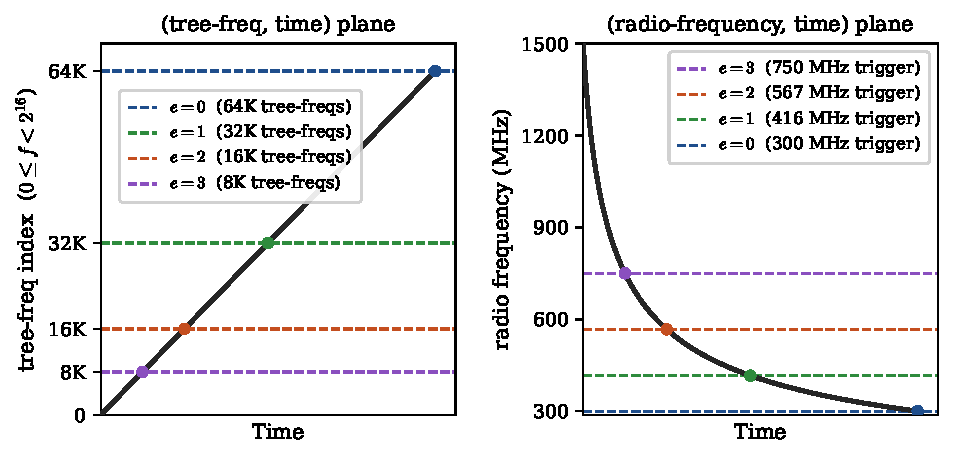
\includegraphics[width=\textwidth]{figs/early_triggers.pdf}
\caption{A visualization of early triggers, in radio frequency (right panel) or the ``tree-freq'' reparametrization used in the code (left panel). Trees with early triggers search the lower part of the tree-freq range, i.e.\ the high part of the radio frequency range. A tree with $e > 0$ triggers earlier (by a factor $2^e$) than the main tree. The plot assumes CHORD params (300--1500 MHz, $r=16$, $0\le e\le 3$).}
\label{fig:early_triggers}
\end{figure}

\begin{figure}[ht]
\centering
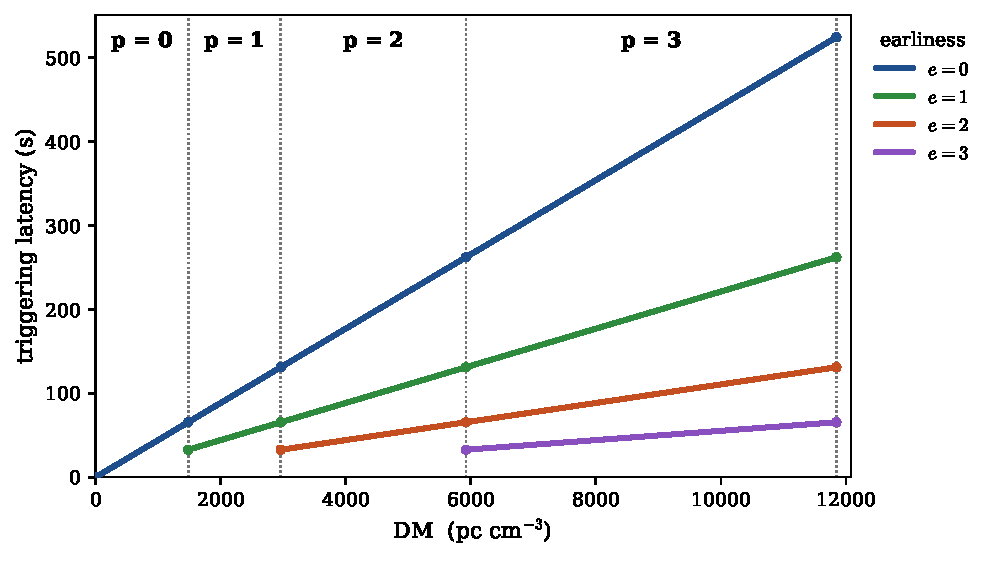
\includegraphics[width=0.85\textwidth]{figs/tree_segments.pdf}
\caption{The ten {\tt DedispersionTrees} from Table\ \ref{tab:chord_sb2_et}, shown as line segments in the (DM, triggering latency) plane. For each tree $(\gamma, e)$, the value of $\gamma$ determines the DM range, and the value of $e$ determines the slope.}
\label{fig:tree_segments}
\end{figure}

\clearpage

\subsection{Dedispersion output arrays}
\label{ssec:dedispersion_output_arrays}

The dedispersion output consists of a pair of 2-d arrays (\verb|out_max|, \verb|out_argmax|)
for each beam and \verb|DedispersionTree|, indexed by {\tt (dm,time)}.
The purpose of this section is to describe these arrays in a little more detail.

\subsubsection{Parameter definitions}

The pirate \verb|DedispersionPlan| defines the following global (i.e.\ not per-tree) parameters:
\begin{align}
T_{\rm in} &= {\tt nt\_in} & \mbox{ (input time samples per time chunk)} \nn \\
r_{\rm top} &= {\tt toplevel\_tree\_rank} & \mbox{ (toplevel tree rank, specified in the config file)} \nn
\end{align}
and the following per-tree parameters:
\begin{align}
\gamma &= {\tt primary\_tree\_index} & \mbox{ (primary tree index; input is time-downsampled by $2^\gamma$)} \nn \\
e &= {\tt early\_trigger\_level}  & \mbox{ (``earliness'' of trigger)} \nn \\
T_{\rm ds} &= {\tt time\_downsampling} & \mbox{ (time coarse-graining factor in peak-finding kernel)} \nn \\
D_{\rm ds} &= {\tt dm\_downsampling}   & \mbox{ (dm coarse-graining factor, denoted $2^{R+K}$ in \S\ref{sec:peak_finding})} \nn
\end{align}
These parameters can be inspected with \verb|pirate_frb show dedisperser -v|, and are also
passed from pirate to the grouper via the \verb|dedispersion_plan| yaml metadata.

{\bf Warning.} Unfortunately, it's not currently possible to choose the coarse-graining factors
$(T_{\rm ds}, D_{\rm ds})$ in the config file! The dedisperser will ``choose them for you'', and 
they need not be the same in all trees. If your downstream code depends on how they're chosen, 
you should put asserts in your code, in case the values change in the future. This is something
I hope to improve soon!

\subsubsection{Output array shapes}

The \verb|out_max| and \verb|out_argmax| arrays (for a fixed tree and beam), have the same
shape $({\tt ndm\_out}, {\tt nt\_out})$, given by:
\begin{align}
{\tt ndm\_out} &= \begin{cases}
  2^{r_{\rm top} - e} / D_{\rm ds} & \mbox{ if } \gamma=0 \\
  2^{r_{\rm top} - e - 1} / D_{\rm ds} & \mbox{ if } \gamma \ge 1
\end{cases} \label{eq:ndm_out} \\
{\tt nt\_out} &= \frac{T_{\rm in}}{2^\gamma T_{\rm ds}} \label{eq:nt_out}
\end{align}
The {\em full-band} delay range searched by each tree (expressed as an integer number samples, 
before any per-tree time downsampling has been done) is:
\begin{equation}
d_{\rm lo} = \begin{cases}
  0 & \mbox{ if } \gamma=0 \\
  2^{r_{\rm top} + \gamma - 1} & \mbox{ if } \gamma\ge 1
\end{cases}
\hspace{1.5cm}
d_{\rm hi} = 2^{r_{\rm top} + \gamma}
\label{eq:dlo_dhi}
\end{equation}
To explain where Eqs.\ (\ref{eq:ndm_out})--(\ref{eq:dlo_dhi}) come from, we walk through steps in the code:
\begin{itemize}

\item On the time axis, we start with a length-$T_{\rm in}$ input array,
  downsample by a factor $2^\gamma$, run tree dedispersion,
  and downsample the output (max-ing, not averaging!) by $T_{\rm ds}$. 
  This implies Eq.\ (\ref{eq:nt_out}).

\item The DM axis is a bit more complicated. First consider the base tree (no downsampling
  or early triggers), and assume $D_{\rm ds}=1$ for simplicity. We have:
  \begin{equation}
   d_{\rm lo} = 0
     \hspace{1.5cm}
   d_{\rm hi} = 2^{r_{\rm top}}
     \hspace{1.5cm}
   {\tt ndm\_out} = 2^{r_{\rm top}}
  \end{equation}
  Then we include additional complications one at a time.
  If we downsample the input by $2^\gamma$, then $d_{\rm hi}$ gets multiplied by $2^\gamma$.
  Recall that for $\gamma > 0$, we also discard the lower half of the output DMs (which was already searched by primary tree $(\gamma-1)$).
  Therefore:
  \begin{equation}
   d_{\rm lo} = \begin{cases}
        0 & \mbox{ if } \gamma = 0 \\
        2^{r_{\rm top} + \gamma - 1} & \mbox{ if } \gamma > 0
   \end{cases}
     \hspace{1cm}
   d_{\rm hi} = 2^{r_{\rm top} + \gamma}
     \hspace{1cm}
   {\tt ndm\_out} = \begin{cases}
     2^{r_{\rm top}} & \mbox{ if } \gamma = 0 \\
     2^{r_{\rm top}-1} & \mbox{ if } \gamma > 0 \\
  \end{cases}
  \end{equation}
  If this is an early-triggered tree with $e > 0$, then the {\em full-band} delay
  range is unchanged, but the spacing between trial DMs increases by $2^e$, so
  {\tt ndm\_out} decreases by the same factor:
  \begin{equation}
   d_{\rm lo} = \begin{cases}
        0 & \mbox{ if } \gamma = 0 \\
        2^{r_{\rm top} + \gamma - 1} & \mbox{ if } \gamma > 0
   \end{cases}
     \hspace{1cm}
   d_{\rm hi} = 2^{r_{\rm top} + \gamma}
     \hspace{1cm}
   {\tt ndm\_out} = \begin{cases}
     2^{r_{\rm top}-e} & \mbox{ if } \gamma = 0 \\
     2^{r_{\rm top}-e-1} & \mbox{ if } \gamma > 0 \\
  \end{cases}
  \end{equation}
  Finally, we downsample the output (max-ing, not averaging!) by $D_{\rm ds}$.
  This decreases {\tt ndm\_out} by a factor $D_{\rm ds}$, leaving $d_{\rm lo}$, $d_{\rm hi}$
  unchanged. This implies Eqs.\ (\ref{eq:ndm_out}), (\ref{eq:dlo_dhi}).
\end{itemize}

\subsubsection{The out\_argmax array}

Each element of the \verb|out_max| array is a ``coarse-grained'' snr value, defined by taking
a maximum over a certain set of parameters: frequency subbands, pulse widths, fine-grained DMs,
and fine-grained arrival times. The \verb|out_argmax| array consists of integer ``tokens''
which encode the ``winning'' parameters, that are responsible for the max snr.

Before writing down the token encoding, recall from \S\ref{sec:peak_finding}, \S\ref{ssec:dedispersion_output_arrays}
that the DM downsampling factor is of the form $D_{\rm ds} = 2^{R+K}$.
The first $R$ bits are part of the ``multiplet'' $0 \le m < M$ (see Eq.\ (\ref{eq:multiplet_def})),
and we introduce a new index $0\le \mu < 2^K$ for the remaining $K$ bits.

In this notation, the token encoding is:
\begin{equation}
\big(\mbox{32-bit {\tt argmax\_token}}\big)
 = \, \mbox{\tt (t) | (p << 8) | (mu << 16) | (m << (16+K))}
\end{equation}
where $0 \le t < T_{\rm ds}$ is an 8-bit fine-grained arrival time, $0 \le p < P$ is
an 8-bit peak-finding profile index (encoding pulse width and profile shape),
$0 \le \mu < 2^K$ is part of the fine-grained DM as defined in the previous paragraph,
and $0 \le m < M \le 114$ is a ``multiplet'' (i.e.~(frequency subband, fine-grained DM) pair).
The arrival time $t$ has a small $p$-dependent time shift applied (see code for details).

In practice, you shouldn't need to know the details of the token encoding -- there are helper
functions that are intended to hide it. In particular, the method \verb|FrbGrouper.create_events()| 
decodes tokens to recover the ``winning'' parameters (min/max freq, DM, timestamp, width) 
for each \verb|out_max| array value.

When using \verb|FrbGrouper.create_events()|, note that the output timestamp is defined to 
be the arrival time at the lowest frequency of the band (400 MHz in CHIME, or 300 MHz 
in CHORD), even if the FRB is detected in a subband.
If there are early triggers, then the timestamp can be {\bf significantly later}
($\sim 10^2$ seconds) than the end of the time-chunk.
With or without early triggers, the timestamp can also be {\bf slightly earlier}
than the beginning of the time-chunk, due to the finite width of the peak-finding
kernels.

\clearpage

\section{Implementation}

\subsection{Non-recursive formulation of tree dedispersion}

Recall from \S\ref{sec:tree_dedispersion} that tree dedispersion $\DD(r)$ is a linear operator
whose inputs and outputs are both $(2^r,N_{\rm time})$, defined recursively via
Eqs.\ (\ref{eq:DD_composition}), (\ref{eq:DD_DS}).
Here, we show that $\DD(r)$ has the following non-recursive definition, where
we sum over frequency channels with lags:
\begin{equation}
{\tt out}[d,t] = \frac{1}{2^{r/2}} \sum_{f=0}^{2^r-1} {\tt in}[f,t - L_r(f,d)]  \label{eq:DD_nonrecursive}
\end{equation}
The ``lag'' function $L_r(f,d)$ is defined by:
\begin{equation}
L_r(f,d) = \sum_{i=0}^{r-1} \sum_{j=0}^{r-1} \Omega_{i+j-r} \, (1-f_i) \, d_j  \label{eq:L_def}
\end{equation}
where $\Omega_n$ is defined by:
\begin{equation}
\Omega_n \equiv \begin{cases}
 2^n & \mbox{if } n \ge 0 \\
  1 & \mbox{if } n = -1 \\
  0 & \mbox{if } n < -1
\end{cases}
\end{equation}
and $f_j,d_j \in \{0,1\}$ are the bits in the base-2 representation:
\begin{equation}
f = \big[ f_{r-1} \cdots f_1 f_0 \big]_2
  \hspace{1.5cm}
d = \big[ d_{r-1} \cdots d_1 d_0 \big]_2
\end{equation}
In Appendix \ref{app:nonrecursive_proof}, we show that the nonrecursive definition 
(\ref{eq:DD_nonrecursive}) of tree dedispersion is equivalent to our previous
recursive definition in Eqs.\ (\ref{eq:DD_composition}), (\ref{eq:DD_DS}).

\subsection{The splitting identity}
\label{ssec:splitting_identity}

The purpose of this section is to explain the following ``splitting identity'':
if $r = r' + r''$, then
\begin{equation}
\DD(r) = \big( \DD(r'') \otimes 1 \big) \circ \LAG\big[ (2^{r''}-1-f'') \, d' \big] \circ \big( 1 \otimes \DD(r') \big)
  \label{eq:splitting}
\end{equation}
where the notation will take a little time to explain.

We split the frequency index $0 \le f < 2^r$ and DM-index $0 \le d < 2^r$ into low/high parts as follows:
\begin{align}
f &= 2^{r'} f'' + f' & \mbox{where } 0 \le f' < 2^{r'} \mbox{ and } 0 \le f'' < 2^{r''} \nn \\
d &= 2^{r''} d' + d'' & \mbox{where } 0 \le d' < 2^{r'} \mbox{ and } 0 \le d'' < 2^{r''} \label{eq:fd_splittings}
\end{align}
Using these splittings, we can view tree dedispersion $\DD(r)$ as a linear operator with
input/output shapes $(2^{r''}, 2^{r'}, N_{\rm time})$.
In the splitting identity (\ref{eq:splitting}), the operators $(\DD(r'') \otimes 1)$
and $(1 \otimes \DD(r'))$ are naturally defined with this array shape.
The middle operator $\LAG\big[ (2^{r''}-1-f'') \, d' \big]$ is defined as follows,
on the same array shape $(2^{r''}, 2^{r'}, N_{\rm time})$.
\begin{equation}
{\tt out}\big[ f'', d', t \big] = {\tt in}\big[f'', d', t - (2^{r''}-1-f'') d' \big]
\end{equation}
Note the asymmetry in the splittings of $f,d$ in Eq.\ (\ref{eq:fd_splittings}): the ``primed''
index $f'$ is the ``fine'' frequency index, whereas the ``primed'' index $d'$ is the ``coarse''
DM-index. This asymmetry arises from the details of the tree dedispersion algorithm. 

One consequence: in implementation, we sometimes end up using bit-reversed DM indices
so that array computations are ``in-place'', rather than via temporary arrays.
(Note that the same phenomenon happens for the FFT algorithm!)
We'll gloss over this detail in the notes, where our goal is to explain the math but
not necessarily the details of the implementation.

When contemplating the splitting identity (\ref{eq:splitting}), the following diagram
may help visualize the RHS:
\begin{equation}
(f,t) \xrightarrow{\rm Reshape} (f'',f',t)
 \xrightarrow{ 1 \otimes \DD(r')} (f'',d',t)
 \xrightarrow{\rm LAG} (f'',d',t)
 \xrightarrow{\DD(r'') \otimes 1} (d'',d',t)
 \xrightarrow{\rm Transpose + Reshape} (d,t)
\end{equation}
where tuples such as $(f'',d',t)$ indicate whether an input/output array is 2-d or 3-d,
and indicate whether each index is interpreted as a frequency or a DM.

We defer the proof of the splitting identity (\ref{eq:splitting}) to 
Appendix \ref{app:splitting_proof}.

\subsection{GPU implementation}
\label{ssec:gpu_implementation}

In this section, we describe our fast GPU implementation of tree dedispersion.
This section is slightly simplified compared to the full implementation, but
accurately captures the ``vibe''.

Our goal is to implement $(1_M \otimes \DD(r))$, where $1_M$ is the identity operator
over a spectator index $0 \le m < M$.
In the text below, we usually streamline notation by omitting the spectator index.
The data is a real-time stream which arrives in ``chunks'' with shape $(M, 2^r, N_{\rm time})$.
The kernel looks like:
\begin{center}
\begin{verbatim}
// Length-M and length-2^r axes have caller-specified strides, time axis has stride 1.
__global__ void dd(float *arr, long mstride, long dstride, float *persistent_state);
\end{verbatim}
\end{center}
The kernel operates in-place (i.e.\ no separate {\tt in} and {\tt out} args).
The ``persistent'' state is a kernel-defined ring buffer that is carried over from one
time chunk to the next (see below).
(Context: we're assuming that as real-time data arrives, the kernel is launched for
$0 \le t < N_{\rm time}$, then launched for $N_{\rm time} \le t < 2N_{\rm time}$, etc.)

For small $r$, we can implement tree dedispersion in a single warp, and launch the
kernel with $M$ warps.
First consider $r=1$. 
From the perspective of a single warp, $\DD(1)$ has input/output shape $(2,N_{\rm time})$
and is defined by:
\begin{align}
{\tt out}[0,t] &= \frac{1}{\sqrt{2}} 
  \big( {\tt in}[0,t] + {\tt in}[1,t] \big) \nn \\
{\tt out}[1,t] &= \frac{1}{\sqrt{2}}
  \big( {\tt in}[0,t-1] + {\tt in}[1,t] \big)
\label{eq:DD1}
\end{align}
This is straightforward to implement in a single warp, but note that we need to save
the value of ${\tt in}[0,N_{\rm time}-1]$ for the next time chunk.
Thus, for $r=1$ the persistent state consists of one element per warp ($M$ elements per kernel).

Next consider a single-warp implementation with $r>1$.
We use the splitting identity (\ref{eq:splitting}) to write:
\begin{equation}
\DD(r) = \underbrace{\big( \DD(1) \otimes 1_{2^{r-1}} \big)}_{\equiv {\mathcal D}_2} 
  \circ \LAG\big[ (1-f'')\, d' \big] 
  \circ \underbrace{\big( 1_2 \otimes \DD(r-1) \big)}_{\equiv {\mathcal D}_1}
\end{equation}
Suppose by induction that we have a single-warp implementation of $\DD(1)$ and $\DD(r-1)$.
The $\LAG\big[\cdots\big]$ operator just means that we put the outputs of ${\mathcal D}_1$
into a logical ring buffer, before feeding them to ${\mathcal D}_2$.
Here, ``logical'' means that the ring buffer is held in registers of a single warp.
This is persistent state: we save the ring buffer to global memory at the end of the kernel, 
and restore it at the beginning of the next kernel.

As $r$ increases, the single-warp implementation eventually becomes impractical.
A little thought shows that the persistent-state size (in elements, not bytes) $P_r$ 
satisfies the recursion:
\begin{equation}
P_r = \underbrace{\Bigg( 2^{r-1} \Bigg)}_{{\mathcal D}_2} 
  + \underbrace{\Bigg( \sum_{d'=0}^{2^{r-1}-1} d' \Bigg)}_{\rm LAG}
  + \underbrace{\Bigg( 2 P_{r-1} \Bigg)}_{{\mathcal D}_1}
\end{equation}
with initial condition $P_1=1$. The solution to this recursion relation is:
\begin{equation}
P_r = 2^{r-2} \big( 2^r + r - 1 \big)  \label{eq:Pr_def}
\end{equation}
Additionally, our implementation uses $2^r$ registers/thread to store a length-32
sliding time window of array values.
Currently, we use the single-warp implementation for $r \le 4$.

To explain the $r > 4$ case, consider $r=8$ for concreteness.
We apply the splitting identity (\ref{eq:splitting}) to write:
\begin{equation}
\DD(8) = \underbrace{\big( \DD(4) \otimes 1_{16} \big)}_{\equiv {\mathcal D}_2}
   \circ \LAG\big[ (15-f'') \, d' \big] 
   \circ \underbrace{\big(1_{16} \otimes \DD(4) \big)}_{\equiv {\mathcal D}_1}
\label{eq:DD8}
\end{equation}
The operators $(\DD(4) \otimes 1_{16})$ and $(1_{16} \otimes \DD(4))$ can be distributed
across 16 warps in a single threadblock (using our single-warp implementation of $\DD(4)$
described above).
In between, we write the data to a ring buffer in {\bf GPU shared memory}, in order to apply 
lags and in order to move data between different warps.
This idea can be applied for any $r$, to obtain a single-threadblock implementation
with one shared memory read/write cycle.

As $r$ increases, the single-threadblock implementation eventually becomes impractical,
due to register and shared memory limits.
The total persistent state size $P_r$ (now interpreted as elements per threadblock) 
is still given by Eq.\ (\ref{eq:Pr_def})\footnote{This is not obvious, but follows from
the following identity: if $r=r'+r''$, then
\begin{equation}
P_r = 2^{r'} P_{r''} + 2^{r''} P_{r'} 
+ \sum_{d'=0}^{2^{r'}-1} \sum_{f''=0}^{2^{r''}-1} (2^{r''}-1-f'') d'
\end{equation}}, but note that the underlying ring buffers
are split between registers and shared memory.
Currently, we use the single-threadblock implementation for $5 \le r \le 8$.

To explain the $r > 8$ case, consider $r=16$ for concreteness.
We use the splitting identity (\ref{eq:splitting}) to write:
\begin{equation}
\DD(16) = \underbrace{\big( \DD(8) \otimes 1_{256} \big)}_{\equiv {\mathcal D}_2}
   \circ \LAG\big[ (255-f'') \, d' \big] 
   \circ \underbrace{\big( 1_{256} \otimes \DD(8) \big)}_{\equiv {\mathcal D}_1}
\label{eq:DD16}
\end{equation}
The operators $(\DD(8) \otimes 1_{256})$ and $(1_{256} \otimes \DD(8))$ can be distributed
across 256 threadblocks in a single kernel (using our single-threadblock implementation 
of $\DD(8)$ described above).

The middle operator $\LAG[\cdots]$ in Eq.\ (\ref{eq:DD16}) is really a no-op.
It just means that we put the outputs of ${\mathcal D}_1$ in a ring buffer in GPU global memory,
before reading them with ${\mathcal D}_2$.
Thus, Eq.\ (\ref{eq:DD16}) tells us how to divide the $\DD(16)$ operation into two GPU kernels,
separated by a ring buffer in {\bf GPU global memory}.
We use this ``two-pass'' implementation of $\DD(r)$ for $9 \le r \le 16$.
(The current code only implements $r \le 16$, but if larger $r$ were needed, then a ``three-pass''
implementation would cover $17 \le r \le 24$.)

In the above implementation, the main idea is to use the splitting identity recursively, to
split tree dedispersion across multiple kernels, then parallelize over threadblocks in a kernel,
then parallelize over threads in a warp.

\subsection{Extracting subbands from a split dedispersion [Claude]}
\label{ssec:subband_extraction}

In \S\ref{sssec:subbanded_dedispersion}, we defined subbanded dedispersion via
a lot of temporary arrays.
In our GPU kernels, we use coalescing tricks to avoid
writing these temporary arrays to global GPU memory (the temporaries exist only in registers).
In this section, we work out the details.

\S\ref{sssec:subbanded_dedispersion} states the construction for a monolithic $\DD(r)$. This
section says what changes when $\DD(r)$ is split as $r = r_0+r_1$ (Eq.\ \ref{eq:splitting},
whose $r',r''$ these are), and is meant to orient a reader before the kernel code.

{\bf Where the subbands are.} A level-$l$ subband is the array after $r-R+l$ steps $\DDS$ in
case 1, or one step earlier plus an explicit merge across the subband midpoint in case 2. The
first stage performs steps $0,\ldots,r_0-1$, so every subband lands in the second stage iff
$R \le r_1$, which {\tt DedispersionConfig::validate()} enforces (its ``Check 2''). Equivalently:
put a $\DD(R)$ at the outside of the second stage, and the level-$l$ subbands are its
intermediates, level $0$ being its input and the full band its output. Being intermediates of a
single stage is what keeps them in registers.

{\bf What lag it needs.} The extraction needs
\begin{equation}
\LAG\big[ (2^R-1-F)\, d_{\rm hi} \big]
\end{equation}
where $0 \le F < 2^R$ is the coarse-freq index (the $f$ of case 1 at $l=0$) and $d_{\rm hi}$ is
the output coarse delay. Given that lag, the $\DD(R)$ which follows produces the $T$'s of cases
1 and 2 by itself, with no further lag logic.

Let $K \equiv r_1 - R$. If $K=0$ the lag above is exactly the $\LAG$ of the $r_0+r_1$ split,
which the implementation applies anyway (a ring buffer in shared memory), so the subband lags
cost nothing. If $K>0$ then $d_{\rm hi} = 2^K d' + \mu$, where $d'$ is the first stage's delay
and $0 \le \mu < 2^K$ comes from an inner $\DD(K)$, and the lag splits as
\begin{equation}
(2^R-1-F)\, d_{\rm hi} = \underbrace{2^K (2^R-1-F)\, d'}_{\mbox{\footnotesize already applied by the $r_0+r_1$ split}}
                        + \underbrace{(2^R-1-F)\, \mu}_{\mbox{\footnotesize one constant per $(F,\mu)$}}
\end{equation}
So $K>0$ costs one compile-time-constant lag per second-stage register, and buys $2^K$ values
of $d_{\rm hi}$ per unit of $d'$.

{\bf Names in the code.} $r_1$ is {\tt dd\_rank1} $= \lceil {\tt dd\_rank}/2 \rceil$, and $K$ is
{\tt DedispersionTree::xdm\_rank()}, the count of ``extra DM'' bits folded into the argmax
token. The kernel is emitted by {\tt cuda\_generator/SbDedisperser.py} and registered by
{\tt GpuSbDedispersionKernel} ({\tt include/pirate/DedispersionKernel.hpp});
{\tt ReferenceTree} is the CPU reference. \S\ref{ssec:subbands_per_tree} says which trees of a
config have $K>0$ (only early-trigger ones).

\subsection{Alignment constraints and the MegaRingbuf}
\label{ssec:dd_alignment}

In the previous section, we stated (just after Eq.\ (\ref{eq:DD16})) that the $\LAG[\cdots]$
operator in global memory is a no-op.
This is a slight simplification: in implementation, we constrain global memory lags to be
128-byte aligned.
(The reason why is a long story -- see the last few paragraphs in this section!)

Let $E$ be the ``segment size'', or the number of data elements per 128-byte cache line:
\begin{equation}
E \equiv \frac{128}{\mbox{\tt sizeof(dtype)}} = \begin{cases}
 32 & \mbox{ for a float32 kernel} \\
 64 & \mbox{ for a float16 kernel}
\end{cases}
\end{equation}
Taking $\DD(16)$ as an example, we split the lag $\lambda(f'',d') = (255-f'') \, d'$ 
appearing in Eq.\ (\ref{eq:DD16}) into ``aligned'' and ``residual'' parts:
\begin{equation}
\lambda(f'',d') \equiv (255-f'') \, d'
  \hspace{1cm}
\lambda_a(f'',d') \equiv E \left\lfloor \frac{\lambda(f'',d')}{E} \right\rfloor
  \hspace{1cm}
\lambda_r(f'',d') \equiv \lambda(f'',d') - \lambda_a(f'',d')
\label{eq:DD16_align}
\end{equation}
We factorize $\DD(16)$ as follows (compare with Eq.\ (\ref{eq:DD16})):
\begin{equation}
\DD(16) =
\underbrace{\big( \DD(8) \otimes 1_{256} \big) 
            \circ \LAG\big[ \lambda_r(f'',d') \big] }_{\equiv {\mathcal D}_2}
   \circ \LAG\big[ \lambda_a(f'',d') \big]
   \circ \underbrace{\big( 1_{256} \otimes \DD(8) \big)}_{\equiv {\mathcal D}_1}
\label{eq:DD16b}
\end{equation}
The residual lag $\lambda_r(f'',d')$ is coalesced into the second-stage
dedispersion kernel ${\mathcal D}_2$ (slightly increasing the size of its persistent
state), and the aligned lag $\lambda_a(f'',d')$ is a no-op in global memory.
The dedispersion kernels have a boolean compile-time parameter \verb|apply_input_residual_lags|
which indicates whether the lag $\lambda_r(f'',d')$ is applied before dedispersion.
(There is a related parameter \verb|input_is_downsampled_tree| which will be explained in
the next section.)

As an aside, something analogous happens internally in the float16 dedispersion
kernels for $5 \le r \le 8$. In this case, recall from the previous section that
we use a single-threadblock, multi-warp kernel with a lagged ring buffer in shared
memory. In order to keep the shared memory IO 32-bit aligned, we split the 16-bit
lag into an even (aligned) part, and a $\{0,1\}$-valued residual part. The shared
memory ring buffer applies the aligned part, and the residual part is coalesced into
the second half of the dedispersion.

Finally, we explain why we constrain global memory lags to be 128-byte aligned.
An obvious reason is that it allows global memory access to be cache-aligned, but
this has a small performance impact.
The larger reason is as follows.

So far, we've stated that intermediate arrays between dedispersion kernels are
stored in a GPU global memory ring buffer.
This is a simplification: we actually store intermediate arrays in the {\tt MegaRingbuf},
a complicated data structure which lives partially in GPU memory, and partially in host
memory.
This is because the total ring buffer size is much larger than GPU memory.
The {\tt MegaRingbuf} is responsible for organizing ring buffer state so that ``short-lag''
elements of the ring buffer stay on the GPU, and ``long-lag'' elements spill to host
memory (in order to minimize PCIe bandwidth).
The {\tt MegaRingbuf} requires 128-byte aligned lags, in order to ensure that all
host-GPU copies are 128-byte aligned.
Here, the alignment really matters -- profiling shows that host-gpu bandwidth is
significantly reduced if addresses are not 128-byte aligned (but does not benefit
from 256-byte alignment).

\subsection{Downsampled trees and the LaggedDownsampler}
\label{ssec:lagged_downsampler}

As mentioned previously (\S\ref{sec:downsampled_early}), for downsampled trees,
we only keep the upper half (in delay $d$) of the dedispersion transform output.
In this section, we explain some tricks to make this more efficient in implementation,
by not computing the lower half, and coalescing kernels.

First we introduce notation for the operator that we want to implement:
\begin{equation}
U \circ \DD(r) \circ \TDS(\gamma)
\end{equation}
The operator $U$ is the ``upper half'' operator whose
input is a shape $(2^r,N_{\rm time}/2^\gamma)$ array and whose output is a shape
$(2^{r-1},N_{\rm time}/2^\gamma)$ array, defined by ${\tt out}[d,t] = {\tt in}[2^{r-1}+d,\,t]$.
The operator $\TDS(\gamma)$ downsamples in time by a factor $2^\gamma$
(with a factor $2^{-\gamma/2}$), i.e.\ it maps a shape $(2^r,N_{\rm time})$ array to a
shape $(2^r,N_{\rm time}/2^\gamma)$ array.

Now consider the following identity (non-obvious, proved in Appendix \ref{app:upper_half_proof}):
\begin{equation}
U \circ \DD(r) = \DD(r-1) \circ \LAG\big[ 2^{r-1} - 1 - f\big] \circ \LS
\label{eq:U_LS}
\end{equation}
Here, $\LS$ is a ``lagged sum'' operator defined as follows. The input is a shape
$(2^r,N_{\rm time}/2^\gamma)$ array, and the output is a shape
$(2^{r-1},N_{\rm time}/2^\gamma)$ array, defined by:
\begin{equation}
{\tt out}[f,t] = \frac{1}{\sqrt{2}} \big( {\tt in}[2f,t-1] + {\tt in}[2f+1,t] \big)
\label{eq:LS_def}
\end{equation}
In implementation, the RHS of Eq.\ (\ref{eq:U_LS}) can be more efficient than the LHS,
since the RHS avoids computing (and throwing away) the lower half of the dedispersion
output (i.e.\ the dedispersion is rank $(r-1)$ instead of rank $r$).

To compute $\DD(r-1)$ on the GPU (for the large $r$-values that arise for CHIME and CHORD),
we apply the splitting identity (\ref{eq:splitting}) to $\DD(r-1)$.
We choose a splitting (note $r-1$ in the leftmost equation):
\begin{equation}
r-1 = r'+r''
  \hspace{1cm}
f = 2^{r'} f'' + f'
  \hspace{1cm}
d = 2^{r''} d' + d''
\end{equation}
and write:
\begin{align}
\DD(r-1)
  &= \big( \DD(r'') \otimes 1 \big)
       \circ \LAG\big[ (2^{r''}-1-f'') \, d' \big] 
       \circ \big( 1 \otimes \DD(r') \big) \\
\LAG\big[ 2^{r-1} - 1 - f\big]
%  &= \LAG\big[ 2^{r'+r''} - 1 - 2^{r'}f'' - f'\big] \nn \\
  &= \LAG\big[ 2^{r'} (2^{r''}-1-f'') \big] \circ \LAG\big[ 2^{r'}-1-f' \big]
\end{align}
In the last line, we have split the lag into two pieces which depend only on
$f''$ and $f'$.
Putting the two equations together, we get:
\begin{equation}
\DD(r-1) \circ \LAG\big[ 2^{r-1} - 1 - f\big] = 
  \big( \DD(r'') \otimes 1 \big)
       \circ \LAG\big[ (2^{r''}-1-f'') \, (d'+2^{r'}) \big]
       \circ \big( 1 \otimes \DD(r') \big)
  \circ \LAG\big[ 2^{r'}-1-f' \big]
\end{equation}
where we used the fact that the operators $\LAG\big[ 2^{r'} (2^{r''}-1-f'') \big]$ and $(1 \otimes \DD(r'))$ commute,
since the lag depends on $f''$ but not $f'$.
Next, we split the leftmost lag on the RHS into aligned and residual parts (as in Eq.\ (\ref{eq:DD16_align})):
\begin{equation}
\lambda(f'',d') \equiv (2^{r''}-1-f'') \, (d'+2^{r'})
  \hspace{1cm}
\lambda_a(f'',d') \equiv E \left\lfloor \frac{\lambda(f'',d')}{E} \right\rfloor
  \hspace{1cm}
\lambda_r(f'',d') \equiv \lambda(f'',d') - \lambda_a(f'',d')
\label{eq:ds_tree_align}
\end{equation}
Putting all of this together:
\begin{align}
U \circ \DD(r) \circ \TDS(\gamma)
  &= 
\underbrace{\big( \DD(r'') \otimes 1 \big) 
            \circ \LAG\big[ \lambda_r(f'',d') \big] }_{\equiv {\mathcal D}_2}
   \circ \LAG\big[ \lambda_a(f'',d') \big]
   \circ \underbrace{\big( 1 \otimes \DD(r') \big)}_{\equiv {\mathcal D}_1} \nn \\
 & \hspace{1cm} \circ \underbrace{\LAG\big[ 2^{r'}-1-f' \big] \circ \LS \circ \TDS(\gamma)}_{\equiv \LDS(r',\gamma)}
  \label{eq:U_DD_TDS}
\end{align}
where the last line defines the ``lagged downsampling kernel'' $\LDS(r',\gamma)$.
As in \S\ref{ssec:dd_alignment}, we coalesce the residual lag $\LAG[\lambda_r(f'',d')]$ into
the second stage dedispersion kernel ${\mathcal D}_2$.
Note however that the form of $\lambda_r(f'',d')$ is different from before (Eqs.\ (\ref{eq:DD16_align}),
(\ref{eq:ds_tree_align}) differ by $d' \rightarrow (d'+2^{r'})$).
The GPU kernel has a boolean argument \verb|input_is_downsampled_tree| to select which residual
lag is applied.

We have now written the downsampled tree $U \circ \DD(r) \circ \TDS(\gamma)$ as the
composition of three kernels $\LDS$, ${\mathcal D}_1$, ${\mathcal D}_2$.
The ``aligned'' lag operator $\LAG[\lambda_a(f'',d')]$ is implemented as a
no-op, using the MegaRingbuf (\S\ref{ssec:dd_alignment}).

For large downsampling factor $\gamma$, the most expensive step in this length-three
chain is the relatively trivial kernel $\LDS(r',\gamma)$, for memory bandwidth reasons:
\begin{itemize}
\item $\LDS(r',\gamma)$ has input shape $(2^r, N_{\rm time})$ and output shape $(2^{r-1}, N_{\rm time}/2^\gamma)$.
\item ${\mathcal D}_1$ and ${\mathcal D}_2$ have input/output shapes $(2^{r-1}, N_{\rm time}/2^\gamma)$.
\end{itemize}
The memory bandwidth requirements are driven by the $\LDS(r',\gamma)$ input array, which
is {\em the same for all $\gamma$}.
Therefore, our ``production'' {\tt LaggedDownsamplingKernel} is a coalesced kernel
which computes $\LDS(r',\gamma)$ for all values of $\gamma$ simultaneously, i.e.\ the
kernel has one input array and $\gamma_{\rm max}$ output arrays.
This coalesced kernel improves performance significantly.

\subsection{Putting it all together: the GPU kernel diagram}
\label{ssec:gpu_kernel_diagram}

In this section, we put everything together, by describing the exact sequence
of GPU kernels in the dedisperser.
We'll also describe a few implementation details that we didn't mention yet
(early trigger implementation, coalesced kernels).
When reading the bullet points below, it may be helpful to refer in parallel
to Figure \ref{fig:gpu_kernels}, which shows the GPU kernel chain visually.

\begin{itemize}

\item
Recall (\S\ref{ssec:splitting_identity}--\ref{ssec:lagged_downsampler}, Eqs.\ (\ref{eq:DD16b}), (\ref{eq:U_DD_TDS}))
that we implement tree dedispersion (at CHIME/CHORD scale) as two kernels, separated by the {\tt MegaRingbuf}.
We'll refer to these kernels as ``stage-1'' and ``stage-2'' kernels.

\item
Recall (\S\ref{sec:downsampled_early}) that some trees may have early triggers, in addition to the ``main'' trigger.
In implementation, all of the triggers for a tree share a stage-1 kernel, but have different stage-2 kernels that
run at different times.
This crucial detail makes early triggers less expensive than might initially be expected.
It complicates the implementation of the {\tt MegaRingbuf}, since each segment in the ring buffer
has one producer and multiple consumers (with different lags).

In general, there is a many-to-one mapping between stage-2 kernels and stage-1 kernels.
We have one stage-1 kernel per primary tree (terminology from \S\ref{sec:downsampled_early}),
and one stage-2 kernel per {\tt DedispersionTree}.

\item 
Recall (\S\ref{sec:peak_finding}, \S\ref{ssec:dedispersion_output_arrays}) that the output of each
stage-2 dedispersion kernel is the input to a peak-finding kernel.
In implementation, we optimize by defining a {\tt CoalescedDdKernel2}, which coalesces the
stage-2 dedispersion kernel and the peak-finding kernel.

\item
The first GPU kernel in Figure \ref{fig:gpu_kernels} is the {\tt TreeGriddingKernel} (denoted {\tt TGK})
which takes a $(N_{\rm freq}, N_{\rm time})$ array to a $(2^r, N_{\rm time})$ array, as described in \S\ref{sec:gridding}.

\item
Next, two kernels operate in parallel: the stage-1 dedispersion kernel (denoted {\tt DD1}) for the base (i.e.\ non-downsampled) tree,
and the {\tt LaggedDownsamplingKernel} ({\tt LDS}), which prepares input for the downsampled (i.e.\ $\gamma \ge 1$) trees.

\item
The {\tt LDS} kernel has $\gamma_{\rm max}$ output arrays (one for each downsampled tree).
Each of these is the input for a distinct {\tt DD1} kernel.

\item
The {\tt DD1} kernels write their output to the {\tt MegaRingbuf}, and each {\tt CoalescedDdKernel2}
(denoted {\tt CDD2} in Figure \ref{fig:gpu_kernels}) reads its input from the {\tt MegaRingbuf}.
Each {\tt CDD2} kernel writes dedispersion output arrays, in the format described in \S\ref{ssec:dedispersion_output_arrays}.

\end{itemize}

\begin{figure}[ht]
\centering
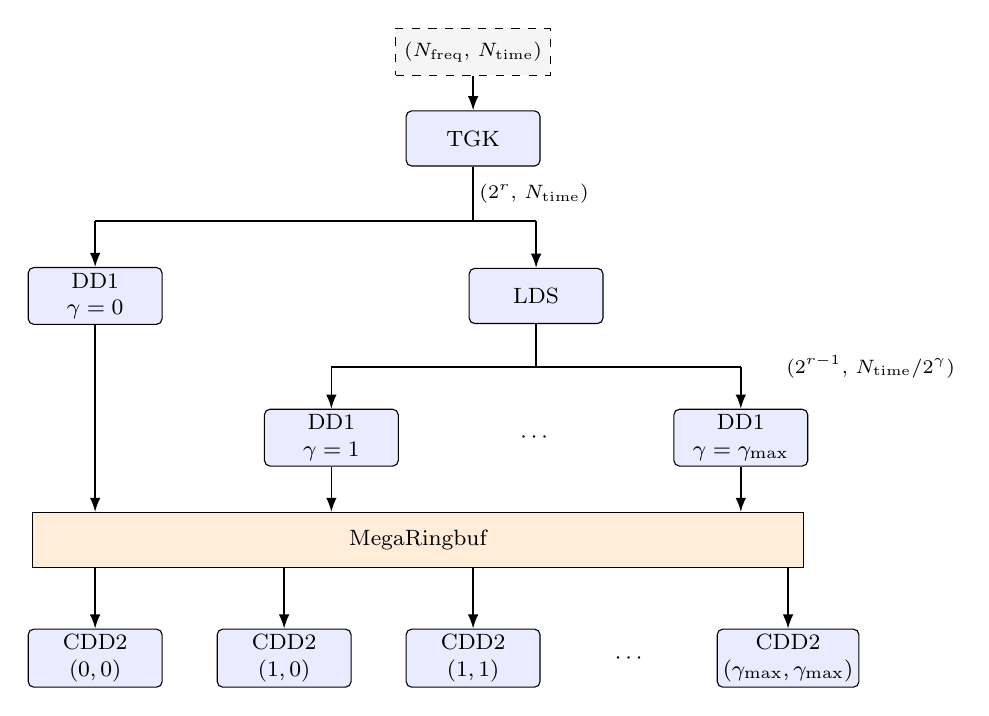
\begin{tikzpicture}[
  font=\footnotesize,
  kern/.style={draw, rounded corners=2pt, fill=blue!8, minimum height=7mm,
               minimum width=17mm, align=center, inner sep=2pt},
  arrn/.style={draw, dashed, fill=black!4, minimum height=6mm, align=center,
               inner sep=3pt, font=\scriptsize},
  ring/.style={draw, fill=orange!15, minimum height=7mm, align=center, inner sep=2pt},
  fl/.style={-{Latex[length=1.8mm]}, semithick},
  sh/.style={font=\scriptsize, inner sep=2pt}
]

% ---------- tree gridding ----------
\node[arrn] (in)  at (0,0)    {$(N_{\rm freq},\,N_{\rm time})$};
\node[kern] (tgk) at (0,-1.1) {TGK};
\draw[fl] (in) -- (tgk);

% ---------- fan-out to the gamma=0 tree, and to the lagged downsampler ----------
\draw[semithick] (tgk) -- node[sh, right] {$(2^r,\,N_{\rm time})$} (0,-2.15);
\draw[semithick] (-4.8,-2.15) -- (0.8,-2.15);

\node[kern] (dd0) at (-4.8,-3.1) {DD1\\$\gamma=0$};
\node[kern] (lds) at ( 0.8,-3.1) {LDS};
\draw[fl] (-4.8,-2.15) -- (dd0);
\draw[fl] ( 0.8,-2.15) -- (lds);

% ---------- one stage-1 dedispersion kernel per downsampling level ----------
\draw[semithick] (lds) -- (0.8,-4.0);
\draw[semithick] (-1.8,-4.0) -- (3.4,-4.0);
\node[sh, anchor=west] at (3.9,-4.0) {$(2^{r-1},\,N_{\rm time}/2^\gamma)$};

\node[kern] (dd1) at (-1.8,-4.9) {DD1\\$\gamma=1$};
\node       (dcd) at ( 0.8,-4.9) {$\cdots$};
\node[kern] (ddg) at ( 3.4,-4.9) {DD1\\$\gamma=\gamma_{\rm max}$};
\draw[fl] (-1.8,-4.0) -- (dd1);
\draw[fl] ( 3.4,-4.0) -- (ddg);

% ---------- MegaRingbuf ----------
\node[ring, minimum width=98mm] (mrb) at (-0.7,-6.2) {MegaRingbuf};
\draw[fl] (dd0) -- (dd0 |- mrb.north);
\draw[fl] (dd1) -- (dd1 |- mrb.north);
\draw[fl] (ddg) -- (ddg |- mrb.north);

% ---------- stage-2 dedispersion + peak-finding, one per (gamma,e) pair ----------
\node[kern] (c00) at (-4.8,-7.7) {CDD2\\$(0,0)$};
\node[kern] (c10) at (-2.4,-7.7) {CDD2\\$(1,0)$};
\node[kern] (c11) at ( 0.0,-7.7) {CDD2\\$(1,1)$};
\node       (ccd) at ( 2.0,-7.7) {$\cdots$};
\node[kern] (cgg) at ( 4.0,-7.7) {CDD2\\$(\gamma_{\rm max},\gamma_{\rm max})$};
\draw[fl] (c00 |- mrb.south) -- (c00);
\draw[fl] (c10 |- mrb.south) -- (c10);
\draw[fl] (c11 |- mrb.south) -- (c11);
\draw[fl] (cgg |- mrb.south) -- (cgg);

\end{tikzpicture}
\caption{The GPU kernels of the dedisperser, and the arrays which connect them.
The labels {\tt TGK}, {\tt LDS}, {\tt DD1}, {\tt CDD2} stand for
{\tt TreeGriddingKernel}, {\tt LaggedDownsamplingKernel},
{\tt GpuDedispersionKernel} (stage 1), and {\tt CoalescedDdKernel2}.
There is one {\tt DD1} kernel per primary tree (or downsampling level $\gamma$),
and one {\tt CDD2} kernel per {\tt DedispersionTree} (or $(\gamma,e)$ pair, where
$e$ is an early trigger level).
Operations internal to the {\tt MegaRingbuf} are not shown (but nontrivial -- they
copy data between the GPU and host, and synchronize with the GPU kernels).
See text in \S\ref{ssec:gpu_kernel_diagram} for more info.}
\label{fig:gpu_kernels}
\end{figure}

\clearpage

\appendix

\section{Derivations [Claude]}
\label{app:derivations}

\subsection{The non-recursive formulation of tree dedispersion}
\label{app:nonrecursive_proof}

In this appendix we prove that the recursive definition of tree dedispersion
(Eqs.\ \ref{eq:DD_composition}, \ref{eq:DD_DS}) is equivalent to the non-recursive definition
(Eq.\ \ref{eq:DD_nonrecursive}), with lag function $L_r(f,d)$ given by Eq.\ (\ref{eq:L_def}).
The proof is by induction on $r$, and uses two structural observations.

\par\noindent
{\bf Observation 1: block structure.}
By inspection of its defining equations, the dedispersion step $\DDS(k)$ computes output
coarse-freq block $f$ using only input blocks $2f$ and $2f+1$, via formulas which do not depend
on $f$ or $r$. Unrolling this over the composition (\ref{eq:DD_DS}): after steps
$\DDS(0), \ldots, \DDS(k-1)$, coarse-freq block $f$ of the intermediate array depends only on
tree-freq channels $2^k f \le (\mbox{tree-freq}) < 2^k (f+1)$, and equals rank-$k$ dedispersion
$\DD(k)$ applied to those $2^k$ channels. In particular, isolating the last step of a
rank-$(r+1)$ composition,
\begin{equation}
\DD(r+1) = \DDS(r) \circ \big( 1 \otimes \DD(r) \big)   \label{eq:app_last_step}
\end{equation}
where we view the rank-$(r+1)$ input array as having shape $(2, 2^r, N_{\rm time})$, and
$(1 \otimes \DD(r))$ applies $\DD(r)$ independently to the lower and upper half-bands
(same tensor notation as in the splitting identity, Eq.\ \ref{eq:splitting}).

\par\noindent
{\bf Observation 2: delay bits.}
By the defining equations of $\DDS(k)$, the output delay is $D = 2\delta + e$, where $\delta$ is
the input delay and $e \in \{0,1\}$ selects the even/odd output line. Thus each step appends one
new low bit to the delay index; at the final step, $D_0 = e$ and $D_j = \delta_{j-1}$ for
$j \ge 1$.

\par\noindent
{\bf Base case.}
For $r=0$, the composition (\ref{eq:DD_DS}) is empty, so $\DD(0)$ is the identity; and
$L_0(0,0) = 0$ is an empty sum, so Eq.\ (\ref{eq:DD_nonrecursive}) reduces to
${\tt out}[0,t] = {\tt in}[0,t]$. (The reader preferring a nontrivial base case may check $r=1$:
$L_1(f,d) = \Omega_{-1} (1-f_0) d_0 = (1-f_0) d_0$, so Eq.\ (\ref{eq:DD_nonrecursive}) reads
${\tt out}[d,t] = 2^{-1/2} \big( {\tt in}[0,t-d] + {\tt in}[1,t] \big)$, which matches $\DDS(0)$
applied to a $(2,1,N_{\rm time})$ input.)

\par\noindent
{\bf Inductive step.}
Assume Eq.\ (\ref{eq:DD_nonrecursive}) holds at rank $r$. By Eq.\ (\ref{eq:app_last_step}) and
the defining equations of $\DDS(r)$ (with coarse output index $f=0$, input delay $\delta$, and
output delay $D = 2\delta + e$):
\begin{equation}
{\tt out}[2\delta+e, t] = \frac{1}{\sqrt{2}}
  \Big( {\tt lo}\big[\delta,\, t - \delta - e\big] + {\tt hi}\big[\delta,\, t\big] \Big)
  \hspace{1.5cm} e \in \{0,1\}
\end{equation}
where ${\tt lo}, {\tt hi}$ denote $\DD(r)$ applied to channels $[0, 2^r)$ and $[2^r, 2^{r+1})$
respectively (the lag $\delta + e$ on the lower block combines the $t-d$ and $t-d-1$ lines).
Substituting the inductive hypothesis,
\begin{equation}
{\tt out}[D, t] = \frac{1}{2^{(r+1)/2}} \left(
  \sum_{g=0}^{2^r-1} {\tt in}\big[g,\ t - \delta - e - L_r(g,\delta)\big]
  + \sum_{g=0}^{2^r-1} {\tt in}\big[2^r + g,\ t - L_r(g,\delta)\big] \right)
\end{equation}
Comparing with Eq.\ (\ref{eq:DD_nonrecursive}) at rank $r+1$, it suffices to prove two
identities for the lag function:
\begin{align}
L_{r+1}(2^r + g,\ D) &= L_r(g, \delta)  \label{eq:app_lag_upper} \\
L_{r+1}(g,\ D) &= L_r(g, \delta) + \delta + e  \label{eq:app_lag_lower}
\end{align}
where (by Observation 2) the bits of $D$ are $D_0 = e$ and $D_j = \delta_{j-1}$ for $j \ge 1$.

To prove Eq.\ (\ref{eq:app_lag_upper}), write $F = 2^r + g$, so that $F_r = 1$ and $F_i = g_i$
for $i < r$. In the double sum
\begin{equation}
L_{r+1}(F, D) = \sum_{i=0}^{r} \sum_{j=0}^{r} \Omega_{i+j-(r+1)} \, (1 - F_i) \, D_j
\end{equation}
the $i=r$ terms vanish, since $(1 - F_r) = 0$. For $i \le r-1$, the $j=0$ term contains
$\Omega_{i-(r+1)}$ with index $i-(r+1) \le -2$, hence also vanishes. Substituting $j = j'+1$ in
the remaining terms gives $\Omega_{i+j'-r} (1-g_i) \delta_{j'}$ summed over
$0 \le i, j' \le r-1$, which is $L_r(g, \delta)$.

To prove Eq.\ (\ref{eq:app_lag_lower}), take $F = g$, so that $F_r = 0$. The $i \le r-1$ terms
give $L_r(g,\delta)$ exactly as before, and the $i = r$ terms contribute
\begin{equation}
(1 - F_r) \sum_{j=0}^{r} \Omega_{j-1} D_j
 = \Omega_{-1} D_0 + \sum_{j=1}^{r} 2^{j-1} D_j = e + \delta
\end{equation}
This completes the induction.

We remark that $\delta + e = \lceil D/2 \rceil$, so Eq.\ (\ref{eq:app_lag_lower}) says that the
lower half-band lags the upper half-band by half of the total delay, rounded up. The case
$\Omega_{-1} = 1$ in the definition of $\Omega_n$ is precisely this round-up -- the algebraic
counterpart of the $(t-d-1)$ in the odd-delay line of $\DDS(k)$.

\subsection{The splitting identity}
\label{app:splitting_proof}

Next we prove the splitting identity (\ref{eq:splitting}), taking the non-recursive definition
(\ref{eq:DD_nonrecursive}) as the starting point. The key statement is an ``additivity''
identity for the lag function: with the index splittings of Eq.\ (\ref{eq:fd_splittings}),
\begin{equation}
L_r(f, d) = L_{r'}(f', d') + (2^{r''} - 1 - f'') \, d' + L_{r''}(f'', d'')
\label{eq:lag_additivity}
\end{equation}

\par\noindent
{\bf Reduction to Eq.\ (\ref{eq:lag_additivity}).}
Expand the right-hand side of the splitting identity (\ref{eq:splitting}) using the
non-recursive form (\ref{eq:DD_nonrecursive}) at ranks $r'$ and $r''$. Acting on an input array
${\tt in}[f'', f', t]$, the three stages give:
\begin{align}
\big( 1 \otimes \DD(r') \big): \hspace{0.5cm}
  A[f'', d', t] &= \frac{1}{2^{r'/2}} \sum_{f'} {\tt in}\big[ f'', f',\ t - L_{r'}(f', d') \big] \nn \\
\LAG: \hspace{0.5cm}
  B[f'', d', t] &= A\big[ f'', d',\ t - (2^{r''}-1-f'') d' \big] \nn \\
\big( \DD(r'') \otimes 1 \big): \hspace{0.5cm}
  C[d'', d', t] &= \frac{1}{2^{r''/2}} \sum_{f''} B\big[ f'', d',\ t - L_{r''}(f'', d'') \big]
\end{align}
Since each stage is a sum of lagged copies of its input, the lags add under composition:
\begin{equation}
C[d'', d', t] = \frac{1}{2^{r/2}} \sum_{f'', f'}
  {\tt in}\Big[ f'', f',\ t - L_{r'}(f',d') - (2^{r''}-1-f'')\,d' - L_{r''}(f'',d'') \Big]
\end{equation}
using $2^{-r'/2}\, 2^{-r''/2} = 2^{-r/2}$. Comparing with $\DD(r)$ in the form
(\ref{eq:DD_nonrecursive}), the splitting identity holds if and only if the total lag above
equals $L_r(f,d)$ for every $(f,d)$ -- i.e.\ if and only if Eq.\ (\ref{eq:lag_additivity})
holds.

\par\noindent
{\bf Proof of Eq.\ (\ref{eq:lag_additivity}).}
Under the splittings (\ref{eq:fd_splittings}), the bits decompose as $f_i = f'_i$ for
$0 \le i < r'$ and $f_{r'+i''} = f''_{i''}$ for $0 \le i'' < r''$; likewise $d_j = d''_j$ for
$0 \le j < r''$ and $d_{r''+j'} = d'_{j'}$ for $0 \le j' < r'$. Now split the double sum
(\ref{eq:L_def}) into four blocks:
\begin{itemize}
\item {\bf (fine freq) $\times$ (low DM):} $i < r'$ and $j < r''$. Here
$i+j-r \le (r'-1) + (r''-1) - r = -2$, so $\Omega_{i+j-r} = 0$ and the block vanishes:
fine-frequency bits never couple to sub-block DM bits.
\item {\bf (fine freq) $\times$ (high DM):} $i < r'$ and $j = r''+j'$. Here
$\Omega_{i+j-r} = \Omega_{i+j'-r'}$, so the block is
$\sum_{i<r'} \sum_{j'<r'} \Omega_{i+j'-r'} (1-f'_i)\, d'_{j'} = L_{r'}(f', d')$.
\item {\bf (coarse freq) $\times$ (low DM):} $i = r'+i''$ and $j < r''$. Here
$\Omega_{i+j-r} = \Omega_{i''+j-r''}$, giving $L_{r''}(f'', d'')$ by the same reindexing.
\item {\bf (coarse freq) $\times$ (high DM):} $i = r'+i''$ and $j = r''+j'$. Here
$i+j-r = i''+j' \ge 0$, so $\Omega$ is in its $2^n$ regime and the block {\em factorizes}:
\begin{equation}
\left( \sum_{i''=0}^{r''-1} 2^{i''} (1 - f''_{i''}) \right)
\left( \sum_{j'=0}^{r'-1} 2^{j'} d'_{j'} \right)
 = (2^{r''} - 1 - f'') \, d'
\end{equation}
which is the $\LAG$ term.
\end{itemize}
Summing the four blocks proves Eq.\ (\ref{eq:lag_additivity}), and hence the splitting
identity.

We remark that each of the three cases in the definition of $\Omega_n$ plays a distinct role
here: the $2^n$ regime produces the factorized cross term (the linear extrapolation of the
coarse-DM slope $d'$ across the $(2^{r''}-1-f'')$ blocks above block $f''$); the shift
invariance of $\Omega_{i+j-r}$ under $(i,j,r) \to (i+a,\, j+b,\, r+a+b)$ makes the two diagonal
blocks reproduce the lower-rank lag functions; and the cutoff $\Omega_n = 0$ for $n \le -2$
expresses the fact that fine-frequency structure never couples to sub-block DM bits. Compare
also the time lags $T$ appearing in the subbanded-dedispersion construction
(\S\ref{sec:subband_search}), which have the same form as the cross term.

\subsection{The upper-half identity}
\label{app:upper_half_proof}

Finally we prove the upper-half identity (\ref{eq:U_LS}), which is what lets a downsampled
tree -- where only the upper half of the DM range is kept -- be computed at rank $(r-1)$
instead of rank $r$. It is a corollary of the splitting identity, so no new computation is
needed: it is the $d'=1$ slice of Eq.\ (\ref{eq:splitting}) at $r'=1$.

Take $r' = 1$ and $r'' = r-1$ in the splittings (\ref{eq:fd_splittings}). The frequency
splitting $f = 2^{r'} f'' + f'$ becomes
\begin{equation}
f = 2 f'' + f'
  \hspace{1.5cm} 0 \le f'' < 2^{r-1}, \quad f' \in \{0,1\}
\end{equation}
so $f''$ indexes a {\em pair} of adjacent tree-freq channels and $f'$ selects a channel within
the pair. The DM splitting $d = 2^{r''} d' + d''$ becomes
\begin{equation}
d = 2^{r-1} d' + d''
  \hspace{1.5cm} d' \in \{0,1\}, \quad 0 \le d'' < 2^{r-1}
\end{equation}
so $d'$ is simply the {\em top bit} of the DM index. Therefore the upper half of the DM range
is exactly the $d'=1$ slice:
\begin{equation}
d \ge 2^{r-1} \iff d' = 1,
  \hspace{1cm}\mbox{and then}\hspace{1cm} d = 2^{r-1} + d''
\end{equation}
i.e.\ $U$ selects $d'=1$, and the surviving DM index of $U \circ \DD(r)$ is $d''$.

With these values, the splitting identity (\ref{eq:splitting}) reads
\begin{equation}
\DD(r) = \big( \DD(r-1) \otimes 1_2 \big)
   \circ \LAG\big[ (2^{r-1}-1-f'') \, d' \big]
   \circ \big( 1_{2^{r-1}} \otimes \DD(1) \big)
\label{eq:uh_splitting}
\end{equation}
on arrays of shape $(2^{r-1}, 2, N_{\rm time})$. Now restrict each of the three factors to
$d'=1$, working right to left:

\begin{itemize}

\item {\bf The $\DD(1)$ factor becomes $\LS$.} The operator $(1 \otimes \DD(1))$ applies
$\DD(1)$ along the length-2 axis, taking $(f'',f',t) \to (f'',d',t)$. By the definition
(\ref{eq:DD1}) of $\DD(1)$, its $d'=1$ output is
\begin{equation}
{\tt out}[f'',1,t] = \frac{1}{\sqrt 2} \big( {\tt in}[f'',0,t-1] + {\tt in}[f'',1,t] \big)
\end{equation}
Since ${\tt in}[f'',0,\cdot]$ and ${\tt in}[f'',1,\cdot]$ are the tree-freq channels $2f''$ and
$2f''+1$, this is precisely the definition (\ref{eq:LS_def}) of $\LS$. (The $d'=0$ output is
the {\em un}lagged sum of the pair, which is what the discarded lower DM-half is built from.)

\item {\bf The $\LAG$ factor becomes $\LAG[2^{r-1}-1-f'']$.} Substituting $d'=1$ into the lag
$(2^{r-1}-1-f'')\,d'$ leaves $(2^{r-1}-1-f'')$, a per-channel lag on the length-$2^{r-1}$ axis.
This is the middle factor of (\ref{eq:U_LS}), with $f''$ playing the role of $f$.

\item {\bf The $\DD(r-1)$ factor is unchanged.} The operator $(\DD(r-1) \otimes 1_2)$ dedisperses
along the $f''$ axis with the $d'$ axis a spectator, so its restriction to the $d'=1$ slice is
just $\DD(r-1)$, taking $f'' \to d''$.

\end{itemize}

\par\noindent
Composing the three restricted factors gives Eq.\ (\ref{eq:U_LS}). As a check on the
normalization, $\LS$ contributes $2^{-1/2}$ and $\DD(r-1)$ contributes $2^{-(r-1)/2}$, for a
total of $2^{-r/2}$, matching $\DD(r)$.

\par\noindent
{\bf The identity at the level of lag functions.} It is worth recording what
(\ref{eq:U_LS}) says about $L_r$, since this is the form in which it is easiest to check.
Writing $f = 2g+b$ with $b \in \{0,1\}$, the additivity identity (\ref{eq:lag_additivity})
at $r'=1$, $d'=1$, $d''=\tilde d$ gives
\begin{equation}
L_r\big(2g+b,\; 2^{r-1}+\tilde d\big)
  = L_{r-1}(g, \tilde d) + \big(2^{r-1}-1-g\big) + (1-b)
\label{eq:uh_lag}
\end{equation}
where we used $L_1(b,1) = \Omega_{-1}(1-b) = 1-b$. Read right to left, the three terms are
exactly the three stages of (\ref{eq:U_LS}): the $\LS$ lag of one sample applied to the even
channel of each pair and none to the odd channel, the $\LAG$ term, and the rank-$(r-1)$ tree.
Note that $(1-b)$ carries no $\tilde d$-dependence -- the lowest frequency bit does not couple
to any DM bit below the top one, by the cutoff $\Omega_n = 0$ for $n \le -2$. That is what makes
the construction possible: within a pair of adjacent tree-freqs, {\em every} DM in the upper half
sees the same one-sample offset, so the pair can be collapsed by $\LS$ before the DM index is
resolved.

\clearpage

\end{document}
